%\documentclass[journal]{IEEEtran}
\documentclass[draftcls,onecolumn,12pt]{IEEEtran}
\IEEEoverridecommandlockouts
%\overrideIEEEmargins

\usepackage[T1]{fontenc}
\usepackage[latin9]{inputenc}
\usepackage[compress]{natbib}
\usepackage{amsthm}
\usepackage{amsmath}
\usepackage{algcompatible}
\usepackage{algorithm}
\usepackage{booktabs}
\usepackage{enumerate}
\usepackage{graphicx}
\usepackage{amssymb}
\usepackage{latexsym}
\usepackage{epstopdf}
\usepackage{color}
\usepackage{bbm}
\usepackage{needspace}
\usepackage{color, colortbl}
\usepackage[english]{babel}
\usepackage{tikz}
\usepackage{caption}
\usepackage{subcaption}
\usetikzlibrary{arrows,automata}
\usetikzlibrary{positioning}
\usepackage{filecontents}

\DeclareCaptionFont{mysize}{\fontsize{8}{9.6}\selectfont}
\captionsetup{font=mysize}

\pagenumbering{gobble}
% *** GRAPHICS RELATED PACKAGES ***
%
\ifCLASSINFOpdf
  % \usepackage[pdftex]{graphicx}
  % declare the path(s) where your graphic files are
  % \graphicsinfectionpath{{../pdf/}{../jpeg/}}
  % and their extensions so you won't have to specify these with
  % every instance of \includegraphics
  % \DeclareGraphicsExtensions{.pdf,.jpeg,.png}
\else
  % or other class option (dvipsone, dvipdf, if not using dvips). graphicx
  % will default to the driver specified in the system graphics.cfg if no
  % driver is specified.
  % \usepackage[dvips]{graphicx}
  % declare the path(s) where your graphic files are
  % \graphicspath{{../eps/}}
  % and their extensions so you won't have to specify these with
  % every instance of \includegraphics
  % \DeclareGraphicsExtensions{.eps}
\fi
% graphicx was written by David Carlisle and Sebastian Rahtz. It is
% required if you want graphics, photos, etc. graphicx.sty is already
% installed on most LaTeX systems. The latest version and documentation can
% be obtained at:
% http://www.ctan.org/tex-archive/macros/latex/required/graphics/
% Another good source of documentation is "Using Imported Graphics in
% LaTeX2e" by Keith Reckdahl which can be found as epslatex.ps or
% epslatex.pdf at: http://www.ctan.org/tex-archive/info/
%
% latex, and pdflatex in dvi mode, support graphics in encapsulated
% postscript (.eps) format. pdflatex in pdf mode supports graphics
% in .pdf, .jpeg, .png and .mps (metapost) formats. Users should ensure
% that all non-photo figures use a vector format (.eps, .pdf, .mps) and
% not a bitmapped formats (.jpeg, .png). IEEE frowns on bitmapped formats
% which can result in "jaggedy"/blurry rendering of lines and letters as
% well as large increases in file sizes.
%
% You can find documentation about the pdfTeX application at:
% http://www.tug.org/applications/pdftex


% *** MATH PACKAGES ***
%
%\usepackage[cmex10]{amsmath}
% A popular package from the American Mathematical Society that provides
% many useful and powerful commands for dealing with mathematics. If using
% it, be sure to load this package with the cmex10 option to ensure that
% only type 1 fonts will utilized at all point sizes. Without this option,
% it is possible that some math symbols, particularly those within
% footnotes, will be rendered in bitmap form which will result in a
% document that can not be IEEE Xplore compliant!
%
% Also, note that the amsmath package sets \interdisplaylinepenalty to 10000
% thus preventing page breaks from occurring within multiline equations. Use:
%\interdisplaylinepenalty=2500
% after loading amsmath to restore such page breaks as IEEEtran.cls normally
% does. amsmath.sty is already installed on most LaTeX systems. The latest
% version and documentation can be obtained at:
% http://www.ctan.org/tex-archive/macros/latex/required/amslatex/math/

\addtolength{\textwidth}{-6mm}
\addtolength{\hoffset}{3mm}
\addtolength{\textheight}{-0mm}
\addtolength{\voffset}{4mm}
\theoremstyle{plain}
\newtheorem{thm}{\protect\theoremname}
  \theoremstyle{plain}
  \newtheorem{lem}[thm]{\protect\lemmaname}
\newtheorem{remark}{Remark}
\newtheorem{coro}{Corollary}
\newtheorem{conjecture}{Conjecture}
\newtheorem{define}{Definition}
\newtheorem{problem}{Problem}


\makeatother

\usepackage{babel}
\providecommand{\lemmaname}{Lemma}
\providecommand{\theoremname}{Theorem}
\newcommand{\norm}[1]{\left\lVert#1\right\rVert}
\renewcommand{\algorithmicrequire}{\textbf{Input:}}
\renewcommand{\algorithmicensure}{\textbf{Output:}}
\newcommand{\Sysbi}{$\mathcal B(\bar A,\bar B)$}
\newcommand{\Digraph}{$G(\bar A,\bar B)$}

\renewcommand{\thesubsubsection}{\alph{subsubsection})}
%\renewcommand{\baselinestretch}{1.5}


\begin{document}
\title{Advanced Lane Finding Project}
\author{Ximing Chen}
\maketitle
\section{Goals and Steps}\label{sec:prelim}
The goals / steps of this project are the following:
\begin{itemize}
\item Compute the camera calibration matrix and distortion coefficients given a set of chessboard images.
\item Apply a distortion correction to raw images.
\item Use color transforms, gradients, etc., to create a thresholded binary image.
\item Apply a perspective transform to rectify binary image ("birds-eye view").
\item Detect lane pixels and fit to find the lane boundary.
\item Determine the curvature of the lane and vehicle position with respect to center.
\item Warp the detected lane boundaries back onto the original image.
\item Output visual display of the lane boundaries and numerical estimation of lane curvature and vehicle position.
\end{itemize}

Here I will consider the rubric points individually and describe how I addressed each point in my implementation.  


\section{Camera Calibration}
I start by preparing ``object points'', which will be the $(x, y, z)$ coordinates of the chessboard corners in the world. Here I am assuming the chessboard is fixed on the $(x, y)$ plane at $z=0$, such that the object points are the same for each calibration image. Thus, object points is just a replicated array of coordinates, and `objpoints` will be appended with a copy of it every time I successfully detect all chessboard corners in a test image.  `imgpoints` will be appended with the $(x, y)$ pixel position of each of the corners in the image plane with each successful chessboard detection. 

In my experiments, I have used a mesh-grid of $n_x = 9$ and $n_y = 6$ to create $54$ object points. The image points are obtained from using the `cv2.findChessboardCorners()' function. Thus, it finds 54 points on the image. Next, I used the output `objpoints` and `imgpoints` to compute the camera calibration and distortion coefficients using the `cv2.calibrateCamera()' function. I applied this distortion correction to the test image using the `cv2.undistort()` function and obtained the following result:
%%%%%%%%%%%%%%%%%%%%%%%%%%%%%%%%% Figure %%%%%%%%%%%%%%%%%%%%%%%%%%%%%%%%%%%%%%%%%%%%%%%
\begin{figure}[htb!!]
    \centering
   \begin{subfigure}[t]{0.45\textwidth}
        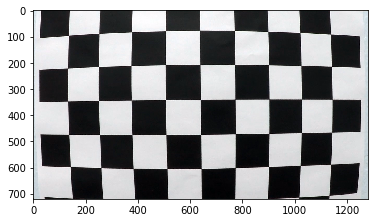
\includegraphics[width=\textwidth]{./figures/chessboard.png}\\
        \caption{}
    \end{subfigure}
    \hspace{-0.5cm}
    \begin{subfigure}[t]{0.45\textwidth}
        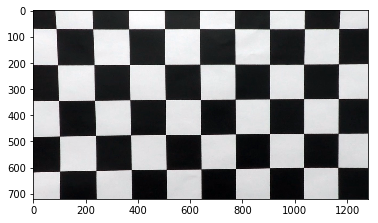
\includegraphics[width=\textwidth]{./figures/undistorted_chessboard.png}\\
        \caption{}
    \end{subfigure}
    \caption{In (a), we show the original image. In (b) we show the undistorted image.}\label{Fig:Chessboard}
\end{figure}

I apply the distortion correction to one of the test images:
\begin{figure}[htb!!]
    \centering
   \begin{subfigure}[t]{0.45\textwidth}
        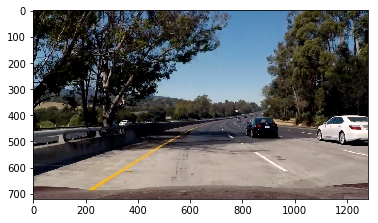
\includegraphics[width=\textwidth]{./figures/test_image.png}\\
        \caption{}
    \end{subfigure}
    \hspace{-0.5cm}
    \begin{subfigure}[t]{0.45\textwidth}
        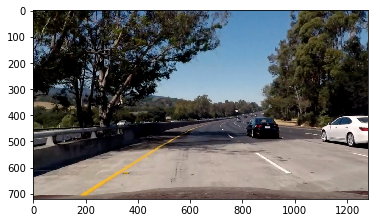
\includegraphics[width=\textwidth]{./figures/test_image_undistort.png}\\
        \caption{}
    \end{subfigure}
    \caption{In (a), we show the original test image. In (b) we show the undistorted test image.}\label{Fig:TestImage}
\end{figure}

\section{Thresholding Color Images}
After the distortion correction process, I begin to apply filters to the color images for better detection of the lanes. I used a combination of color and gradient thresholds to generate a binary image. To get which filter combinations work the best, I use one of the test images, as depicted in Figure~\ref{Fig:TestImage}-(a). 

First, I transform the image from RGB domain to HLS domain. The reason for this is that the lanes usually have high satuation values despite they may have different colors. Thus, HLS domains are more robust hence more suitable for our goal. We use a threshold for the S-channel. More specificially, only the pixel values within the range $[thresh low, thresh high]$ are taken, otherwise they will be set to 0. The $S$-channel is shown as follows:
\begin{figure}[htb!!]
    \centering
   \begin{subfigure}[t]{0.3\textwidth}
        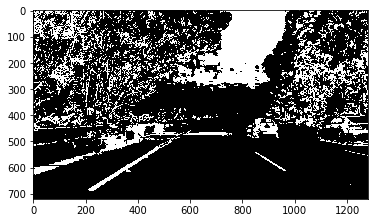
\includegraphics[width=\textwidth]{./figures/schannel100.png}\\
        \caption{}
    \end{subfigure}
    \hspace{-0.5cm}
    \begin{subfigure}[t]{0.3\textwidth}
        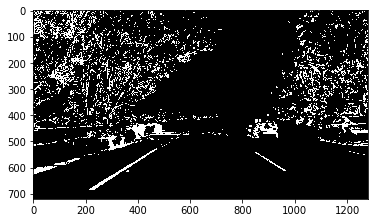
\includegraphics[width=\textwidth]{./figures/schannel.png}\\
        \caption{}
    \end{subfigure}
        \begin{subfigure}[t]{0.3\textwidth}
        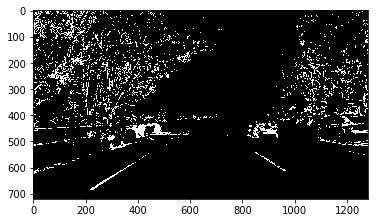
\includegraphics[width=\textwidth]{./figures/schannel200.png}\\
        \caption{}
    \end{subfigure}
    \caption{In (a), the thresh is set to be $[100, 255]$. In (b), the threshold is $[150, 255]$. In (c), the threshold is $[200, 255].$}\label{Fig:Schannel}
\end{figure}
We observed that the best threshold is around $150.$ In this case, we preserve most of the details on the lanes while removing unnecessary information, e.g., the sky as in Figure~\ref{Fig:Schannel}-(a).

Nonetheless, using only the S channel is not enough to provide good quality of the lanes. Thus, we consider the following three additional steps. First, we apply a sobel filter -- a filter typically used to detect the edges -- on the $x$ and $y$-direction of the image, respectively. The performance is shown as follows: 
\begin{figure}[htb!!]
    \centering
   \begin{subfigure}[t]{0.45\textwidth}
        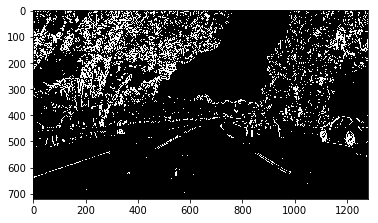
\includegraphics[width=\textwidth]{./figures/sobelx.png}\\
        \caption{}
    \end{subfigure}
    \hspace{-0.5cm}
    \begin{subfigure}[t]{0.45\textwidth}
        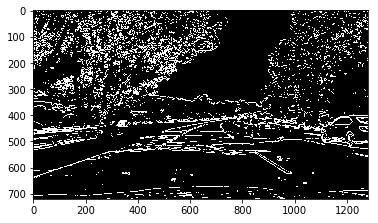
\includegraphics[width=\textwidth]{./figures/sobely.png}\\
        \caption{}
    \end{subfigure}
    \caption{In (a), we show the sobel x filtered image with threshold $(20, 255)$. In (b), we show the sobel y filtered image with threshold $(20, 255).$}\label{Fig:Sobel}
\end{figure}
Notice that sobel-$x$ performs much better than sobel-$y.$ This is due to most of the lanes are perpendicular to the bottom-most boundary of the image. Consequently, the lane colors have high value changes on the $x$ direction. The threshold are obtained using trail-and-error.

We then combine the $S$-channel information with the binary image obtained using sobel-$x$ filter. However, this combination is unable to remove the shadows on the road, no matter how the thresholds are tuned, as shown in Figure~\ref{Fig:FilterFinal}-(a). To address this issue, we use the $L$-channel. The intuition behind this is that the lanes are usually of higher light intensity than the shadows. Thus, we aim to select the `light' and `highly saturated' areas.

\begin{figure}[htb!!]
    \centering
   \begin{subfigure}[t]{0.45\textwidth}
        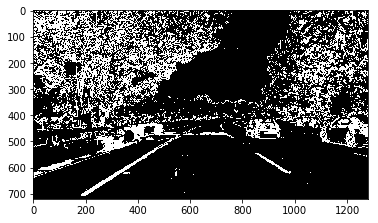
\includegraphics[width=\textwidth]{./figures/color_gradient.png}\\
        \caption{}
    \end{subfigure}
    \hspace{-0.5cm}
    \begin{subfigure}[t]{0.45\textwidth}
        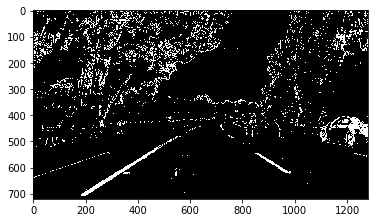
\includegraphics[width=\textwidth]{./figures/color_gradient_light.png}\\
        \caption{}
    \end{subfigure}
    \caption{In (a), we show the figure obtained using $HLS$ and sobel-$x.$ In (b), we show the sobel y filtered image using $S$-channel, $L$-channel and sobel-$x.$}\label{Fig:FilterFinal}
\end{figure}

\section{Perspective Transform}
The code for my perspective transform includes a function called `perspective transform()', in the 10-th code cell of the IPython notebook.  The function takes an image, as well as source (`src') and destination (`dst') points. I chose the hardcode the source and destination points in the following manner:

\begin{verbatim}
offset = 150
left_bottom_x = 160
right_bottom_x = 1150
left_top_x = 585
right_top_x = 705
src = np.float32([[left_top_x, 455], [right_top_x, 455], 
[right_bottom_x, 720], [left_bottom_x, 720]])
dst = np.float32([[left_bottom_x + offset, 0], 
[right_bottom_x-offset, 0],
[right_bottom_x-offset, img_size[0]], 
[left_bottom_x + offset, img_size[0]]])
\end{verbatim}

This results in the following transformation:
\begin{table}[!h]
\centering
\begin{tabular}{@{} *2l @{}}    \toprule
\emph{Source} & \emph{Destination} \\ \midrule
(585, 455)  & (310, 0) \\  \hline
(705, 455)  &  (1000, 0)\\  \hline
(1150, 720)  &  (1000, 720)\\  \hline
(160, 720)  &  (310, 720)\\  \bottomrule \hline
\end{tabular}\caption{This table shows the source and destination point of perspective transform.}\label{Tab:PerspectiveTransform}
\end{table}

\begin{figure}[htb!!]
    \centering
   \begin{subfigure}[t]{0.3\textwidth}
        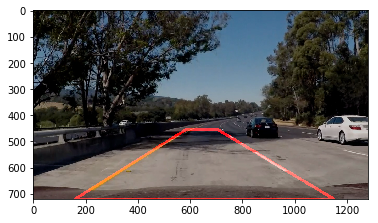
\includegraphics[width=\textwidth]{./figures/SelectedRegion.png}\\
        \caption{}
    \end{subfigure}
    \hspace{-0.5cm}
    \begin{subfigure}[t]{0.3\textwidth}
        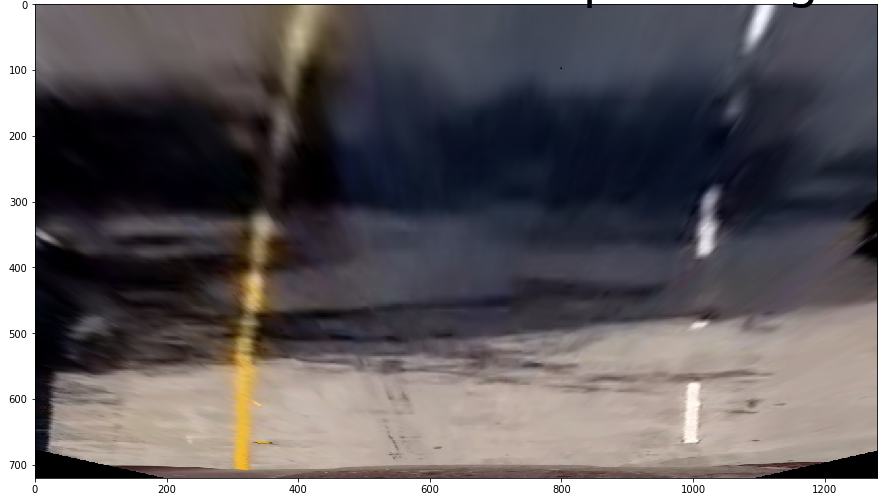
\includegraphics[width=\textwidth]{./figures/Warped_color.png}\\
        \caption{}
    \end{subfigure}
        \begin{subfigure}[t]{0.3\textwidth}
        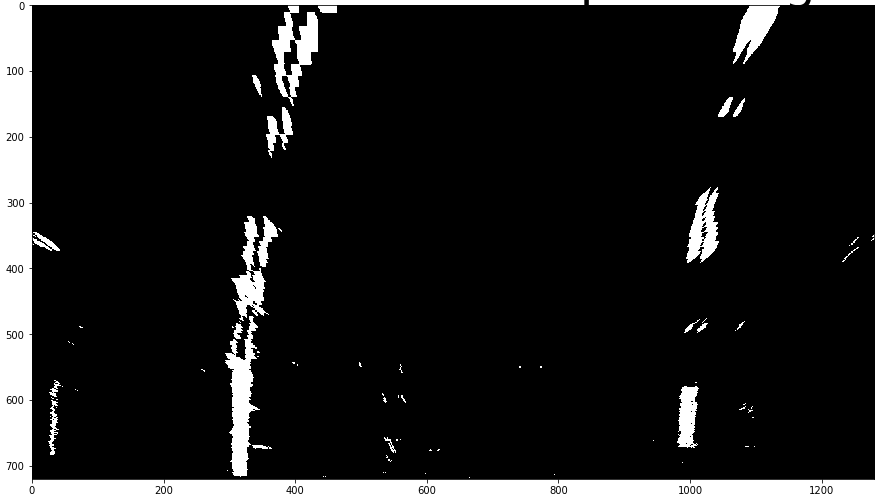
\includegraphics[width=\textwidth]{./figures/Warped.png}\\
        \caption{}
    \end{subfigure}
    \caption{(a) selected region. In (b), the bird-eye-view of the road is shown. In (c), the undistorted warped lanes are shown.}\label{Fig:Warp}
\end{figure}

I verified that my perspective transform was working as expected by drawing the `src` and `dst` points onto a test image and its warped counterpart to verify that the lines appear parallel in the warped image, see Figure~\ref{Fig:Warp} for more details.

\section{Lane Pixel Detection and Fitting}
To detect lane pixels, I basically follow the following steps:
\begin{enumerate}
\item Plot the histogram of the number of pixels across different $x$-positions using only bottom half of the images;
\item Identify the peaks of the histogram iteratively using sliding windows, in this project, we have used 9 windows in total.
\end{enumerate}

To fit the polynomial, I used the `np.polyfit()' function in which the arguments are the identified pixel locations corresponding to the lanes in $y$-direction and in $x$-direction respecitvely. The degree of the polynomial considered equals to 2. The identified polynomial is shown below:

\begin{figure}[htb!!]
    \centering
   \begin{subfigure}[t]{0.5\textwidth}
        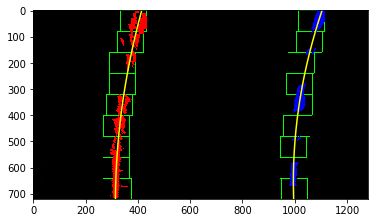
\includegraphics[width=\textwidth]{./figures/Polyfit.png}\\
    \end{subfigure}
    \caption{The sliding windows and the fitted polynomial}\label{Fig:PolyFit}
\end{figure}

\section{Calculations}
We calculated two related information: the curvature and the difference with respect to the center of the lanes.

The curvature is calculated as follows:
\begin{equation}
R = \frac{(1 + (2Ay + B)^2)^{\frac{3}{2}}}{|2A|},
\end{equation}
where $A, B$ are the coefficients of the fitted polynomial $f(x) = Ax^2 + Bx +C.$ The value $y$ is chosen to be equal to the size of the image, as we are interested in the curvature of the lane at the front of the car. However, the calculated curvature is in the pixel-unit, instead of in meters. Thus, we consider doing the following remaping and recalculation.

First, we re-estimate the coefficients of polynomials. This is achieved by scaling the pixel locations by the following factors: $x_f = \frac{3.7}{700}$ and $y_f = \frac{30}{720},$ i.e., $x_f$ represents $3.7$ meters per $700$ pixels. Then, we can calculate the curvature using the above formula, where $A, B$ are the coefficients of polynomial fitted using scaled units and $y$ equals to the size of the image times the scaling factor $y_f.$

Similarly, to get the difference with respect to the center of the lanes. We first identify the location of two lanes -- in meters unit. Then, the center of the lane equals to the average of these two values, whereas the center of the car equals to $640 * x_f$ (meters), since the width of the image is $1280$ pixels. Then, the difference is the mid position minus the center of the car.

I coded these logics in the functions: `get bias()' and `set curvature' in the Line class.

\section{Remapped Image}
Finally, I mapped the identified polynomials into the original image using inverse-perspective transformation and annotate the image, as 

\begin{figure}[htb!!]
    \centering
   \begin{subfigure}[t]{0.45\textwidth}
        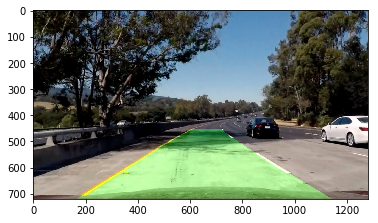
\includegraphics[width=\textwidth]{./figures/Mapped.png}\\
        \caption{}
    \end{subfigure}
    \hspace{-0.5cm}
    \begin{subfigure}[t]{0.45\textwidth}
        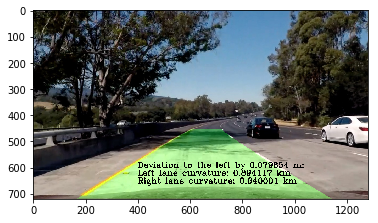
\includegraphics[width=\textwidth]{./figures/Annotated.png}\\
        \caption{}
    \end{subfigure}
    \caption{}\label{Fig:FilterFinal}
\end{figure}

\section{Video}
Please see the zip file for video.

\section{Discussion}
The performance of the lane tracking mostly relies on how good the filters are. When the filter cannot efficiently distinguish what are the pixels corresponding to the lanes, then all following work may be useless. In this case, simply using HLS and sobel filter may not be enough. There are a few instance when this fails: (i) lack of samples, which occurs when another car in front is changing lanes into ours, resulting in blocking the lanes, and (ii) poor samples, the lanes are not colored well. We may consider using prediction from the previously identified polynomials since the lanes are almost continuous, thus, they must follow relatively good geometric shape. 

Also, if the driver changes a lane, then our method may fail to work since we have assumed that there are only left, and right lane on the road. To make it more robust, it is necessary to consider using a non-static method to add lanes into the image, for example, we plot all the lanes detected into the figure.
\end{document}

